\chapter{Making Accessible Tables}
\section{Simple Examples}
%Here is a very basic table.
A very basic table is given in Table~\ref{table:simple}.
The key points about making tables accessible are the following: we must have a header row and we need to specify where it is located (\textit{cf.} the source for \autoref{table:simple}).
Moreover, to make the table easily navigable on screen readers, we require every table to be \textit{regular} in the sense that each row has the same number of columns and \textit{vice versa}.
Finally, we require that every cell be nonempty.
As far as general formatting is concerned, a table's caption must be located \textit{above} its contents (in contrast with a figure) and, as with figures and equations, all tables should be referenced in the text.

\begin{table}[h]
  \centering
  \caption{A simple table}
  \label{table:simple}
  \tagpdfsetup{table/header-rows={1}}
  \begin{tabular}{rccc} \toprule
    \# cells & h & $L^2$ error & rate \\ \midrule
    \num{12} & \num{8.250e-2} & \num{2.945e-3} & -- \\
    \num{25} & \num{3.960e-2} & \num{7.878e-4} & \num{1.80} \\
    \num{50} & \num{1.980e-2} & \num{2.128e-4} & \num{1.89} \\
    \num{100} & \num{9.900e-3} & \num{5.507e-5} & \num{1.95} \\
    \num{200} & \num{4.950e-3} & \num{1.395e-5} & \num{1.98} \\
    \num{400} & \num{2.475e-3} & \num{3.522e-6} & \num{1.99} \\
    \num{800} & \num{1.238e-3} & \num{9.041e-7} & \num{1.96} \\
    \num{1600} & \num{6.188e-4} & \num{2.489e-7} & \num{1.86} \\
    \bottomrule
  \end{tabular}
\end{table}

Observe in the source (\texttt{chapters/making-tables.tex}) that \autoref{table:input} is \texttt{input} from a file in the \texttt{tables} directory.
This is a helpful strategy for organizing and maintaining large projects such as your thesis.
The documentation for making tables in a tagged PDF can be found in the \href{https://texdoc.org/serve/latex-lab-table/0}{latex-lab-table package manual}.

\begin{table}
  \begin{center}
    \caption{Another table, this time \texttt{input} from a separate file}
    \label{table:input}
    \tagpdfsetup{table/header-rows={1}}
    \begin{tabular}{rccc} \toprule
      \# cells & h & $L^2$ error & rate \\ \midrule
      $25$ & $3.960\times10^{-2}$ & $3.100\times10^{-3}$ & -- \\
      $50$ & $1.980\times10^{-2}$ & $1.101\times10^{-3}$ & $1.49$ \\
      $100$ & $9.900\times10^{-3}$ & $4.156\times10^{-4}$ & $1.40$ \\
      $200$ & $4.950\times10^{-3}$ & $2.001\times10^{-4}$ & $1.05$ \\
      $400$ & $2.475\times10^{-3}$ & $8.739\times10^{-5}$ & $1.20$ \\
      $800$ & $1.238\times10^{-3}$ & $4.199\times10^{-5}$ & $1.06$ \\
      $1600$ & $6.188\times10^{-4}$ & $1.979\times10^{-5}$ & $1.09$ \\
      $3200$ & $3.094\times10^{-4}$ & $9.716\times10^{-6}$ & $1.03$ \\
      \bottomrule
    \end{tabular}
  \end{center}
\end{table}


\newpage

\section{Using Table Environments Without Tagging}

Here, we use a \texttt{tabular} environment just to align some content.
This might occur if you want to align figures side-by-side or in a grid, as demonstrated in \autoref{fig:side-by-side} for example.
In this case, we need to tell \LaTeX\ not to tag this as a table, since it really does not \textit{function} as a table (it is merely decorative).
We do so with an option in the place where you would otherwise need to specify the header location.
As an aside, this example also shows how to leave an abridged caption inside the List of Figures.
\vspace{3em}

\begin{figure}[ht]
  \centering
  \tagpdfsetup{table/tagging=false}
  \setlength{\tabcolsep}{40pt}
  \begin{tabular}{cc}
    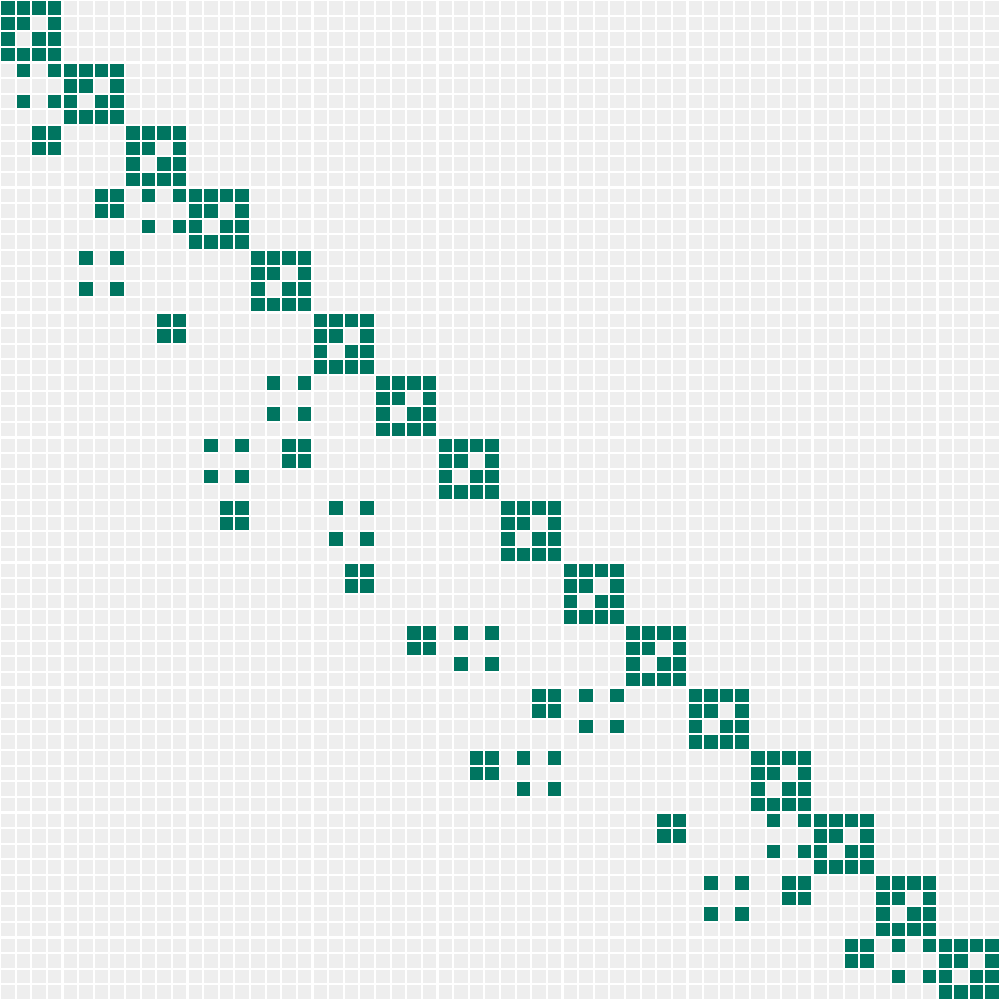
\includegraphics[height=5cm,alt={Sparsity pattern from a discontinuous Galerkin method, demonstrating a lower block-triangular structure.}]{figs/example-a.pdf}
    &
    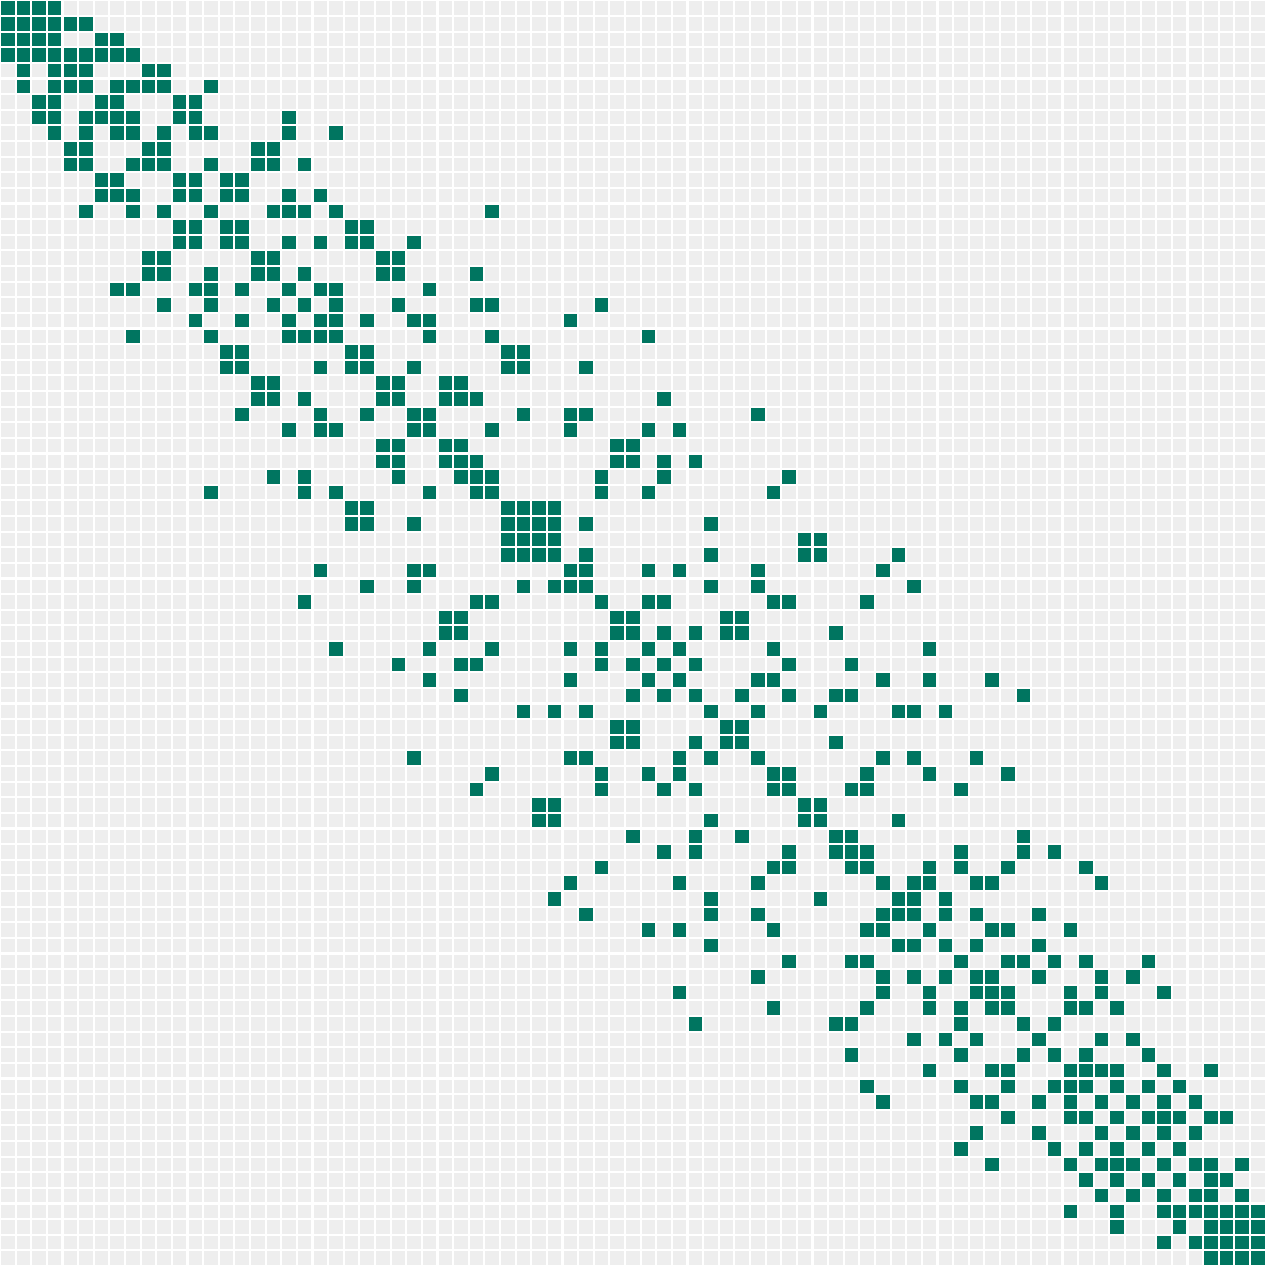
\includegraphics[height=5cm,alt={Sparsity pattern from the SUPG method, demonstrating a sparse, banded structure.}]{figs/example-b.pdf}
  \end{tabular}
  \caption[Comparison of dG/SUPG sparsity patterns]{Comparison of dG/SUPG sparsity patterns. Sparsity patterns for the dG method with upwind flux (left) and the SUPG method (right).}
  \label{fig:side-by-side}
\end{figure}
